\chapter{SINTESI SOTTRATTIVA}
\section*{Sintesi Sottrattiva}

\begin{itemize}
    \item segue l’idea duale
    \item suono ricco spettralmente
    \item elementi fondamentali:
    \begin{itemize}
        \item Oscillatori
        \item Filtri
    \end{itemize}
    \item nata nel mondo analogico
\end{itemize}

Il pilotaggio di segnali è associato a valori controllati di tensioni e correnti.

Nella maggior parte dei sintetizzatori si usa la combinazione VCO (Voltage Controlled Oscillator), VCF (Voltage Controlled Filter), VCA (Voltage Controlled Amplifier) per pilotare gli elementi tempo-varianti.

\begin{figure}[H]
    \centering
    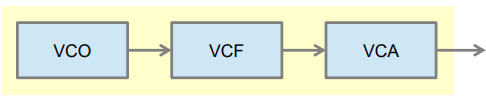
\includegraphics[width=0.7\textwidth]{capitoli/capitolo12/immagini/image1.png}
\end{figure}

\section{Generatori di Rumore}

I rumori possono essere:
\begin{itemize}
    \item Bianchi
    \item Rosa
    \item Marroni
\end{itemize}

\begin{figure}[H]
    \centering
    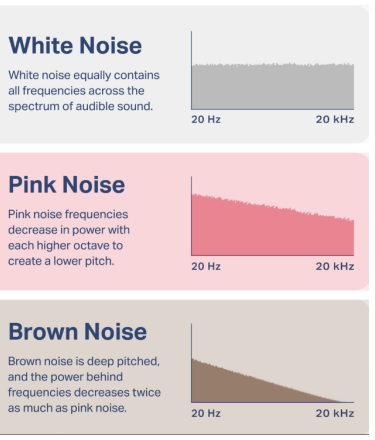
\includegraphics[width=0.7\textwidth]{capitoli/capitolo12/immagini/image2.png}
\end{figure}

Il "colore" del rumore definisce la pendenza di attenuazione dell’energia in funzione della frequenza.

\section{Transistor Ladder Filter (Lowpass)}

\begin{itemize}
    \item basato su una topologia \textit{ladder}
    \item utilizza coppie di transistor differenziali
    \item 4 poli (di solito)
    \item retroazione complessa $\rightarrow$ in tempo discreto si traduce in loop privi di ritardo
    \item può essere altamente non lineare
\end{itemize}
\vspace{8cm}
\section{Sallen-Key Filter}

\begin{itemize}
    \item filtri attivi RC del secondo ordine
    \item non richiedono induttori
    \item realizzati con una cascata di filtri
    \item evitano problemi di sincronizzazione
\end{itemize}

Topologia passa-basso molto comune.

\begin{figure}[H]
    \centering
    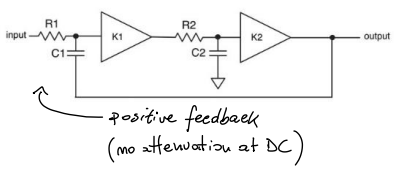
\includegraphics[width=0.7\textwidth]{capitoli/capitolo12/immagini/image3.png}
\end{figure}

\section{State Variable Filter}

\begin{itemize}
    \item composto da due integratori e una retroazione
    \item filtro multimodale
    \item utilizza retroazione negativa
    \item può essere usato come risonatore del secondo ordine perchè il segnale può essere molto basso
\end{itemize}

\begin{figure}[H]
    \centering
    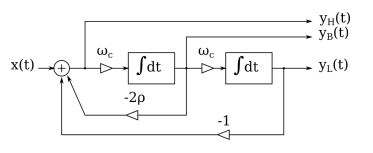
\includegraphics[width=0.7\textwidth]{capitoli/capitolo12/immagini/image4.png}
\end{figure}
\vspace{8cm}
\section{Voltage Controlled Amplifier (VCA)}

\begin{itemize}
    \item controllo dell’ampiezza per aggiungere dinamismo al suono
    \item permette di imitare strumenti acustici
    \item necessita di un generatore di inviluppo (EG / ADSR):
    \begin{itemize}
        \item produce tensione di controllo per impostare l’ampiezza del VCA
        \item i segmenti dell’inviluppo sono:
        \begin{itemize}
            \item \textbf{Attack}
            \item \textbf{Decay}
            \item \textbf{Sustain}
            \item \textbf{Release}
        \end{itemize}
    \end{itemize}
\end{itemize}

\begin{figure}[H]
    \centering
    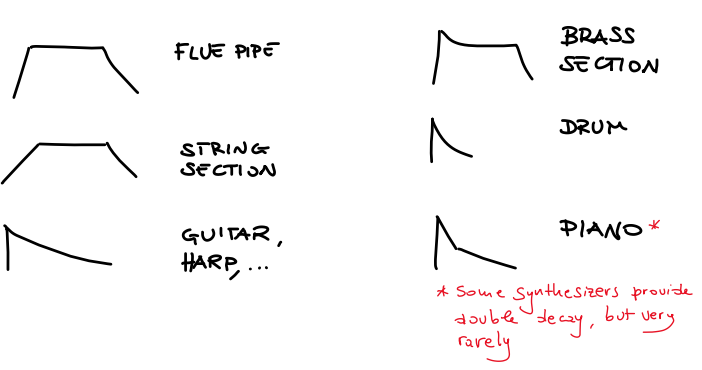
\includegraphics[width=0.7\textwidth]{capitoli/capitolo12/immagini/image5.png}
\end{figure}